\section{Secret Key Encryption}

%%%%%%%%%%%%%%%%%%%%%%%%%%%%%%%%%%%%%%%%%%%%%%%%%%%%%%%%%%%%%%%%%%%%%%%%%%%%%%%%
\subsection{Encryption using Different Ciphers and Modes}

For this section, I used 3 different ciphers in different modes. 
They are
\begin{enumerate}
    \item Block cipher AES in CFB mode, where key length is 256.
    \item Block cipher SM4 in CTR mode.
    \item Stream cipher RC4.
\end{enumerate}%

Commands used is screenshot as Fig.\ref{fig:p1_1}:

\begin{figure}[hb]
\centering
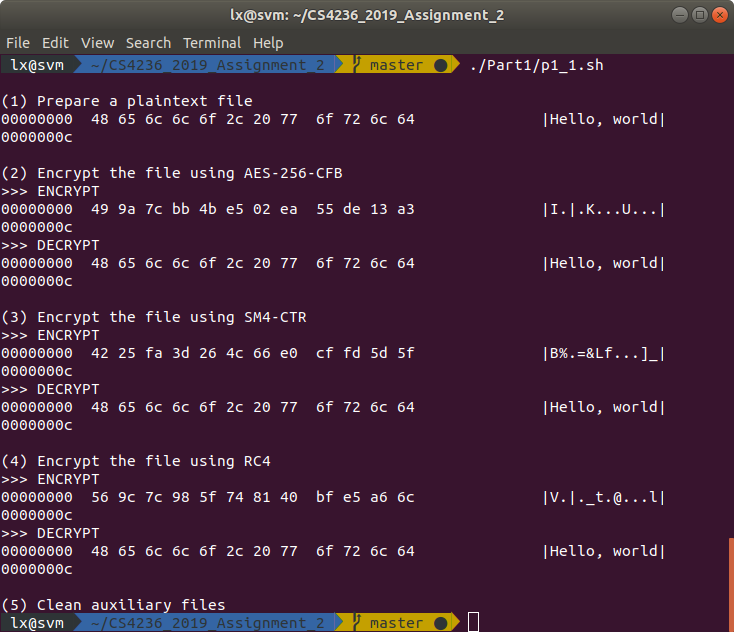
\includegraphics[width=\columnwidth]{resources/p1_1.png}
\caption{
    Content in file \texttt{Part1/p1\_1.sh} is listed in Appendix \ref{code:1_1}
}
\label{fig:p1_1}
\end{figure}

%%%%%%%%%%%%%%%%%%%%%%%%%%%%%%%%%%%%%%%%%%%%%%%%%%%%%%%%%%%%%%%%%%%%%%%%%%%%%%%%
\subsection{Encryption Mode – ECB vs. CBC}

\begin{figure}[t!]
\centering
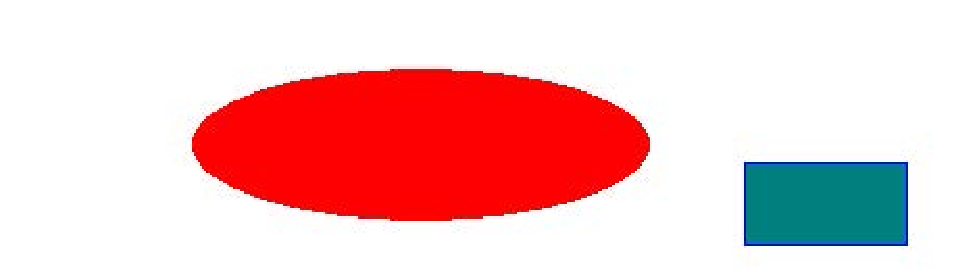
\includegraphics[width=\columnwidth]{resources/pic_original.pdf}
\caption{
    The original picture
}
\label{fig:pic_original}
\end{figure}

\begin{figure}[t!]
\centering
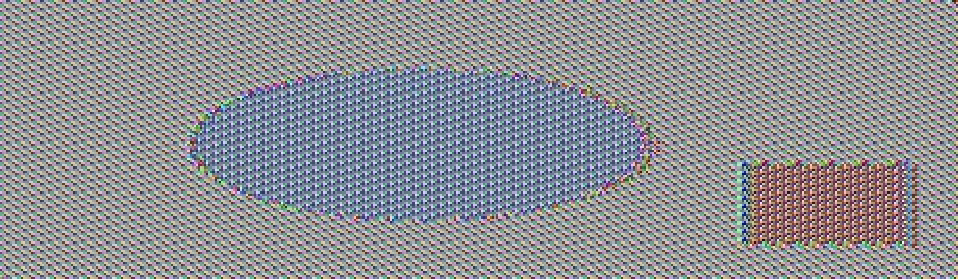
\includegraphics[width=\columnwidth]{resources/pic_ecb.pdf}
\caption{
    The picture encrypted in ECB mode.
}
\label{fig:pic_ecb}
\end{figure}

\begin{figure}[t!]
\centering

\includegraphics[width=\columnwidth]{resources/pic_cbc.pdf}
\caption{
    The picture encrypted in CBC mode.
}
\label{fig:pic_cbc}
\end{figure}

From the ECB-encrypted picture (Fig.\ref{fig:pic_ecb}), we can clearly see the edges of the graphics.
While from the CBC-encrypted picture (Fig.\ref{fig:pic_cbc}), we can hardly find any information.

Using ECB mode merely concatenates the output of the block cipher as the ciphertext. 
That is, the same blocks of plaintext was mapped to the same ciphertext.
We don't change the relative position of blocks either. Consequently, the shape information was almost completely preserved. 

In CBC mode, each block of plaintext is firstly XOR-ed with the previous block of ciphertext. Therefore, identical blocks are encoded as different ciphertext. So the shape information was well hidden. 

%%%%%%%%%%%%%%%%%%%%%%%%%%%%%%%%%%%%%%%%%%%%%%%%%%%%%%%%%%%%%%%%%%%%%%%%%%%%%%%%
\subsection{Initialization Vector (IV)}

\subsubsection{}

Screenshot of the commands and outputs is as Fig.\ref{fig:p1_3_1}.

\begin{figure}[t!]
\centering
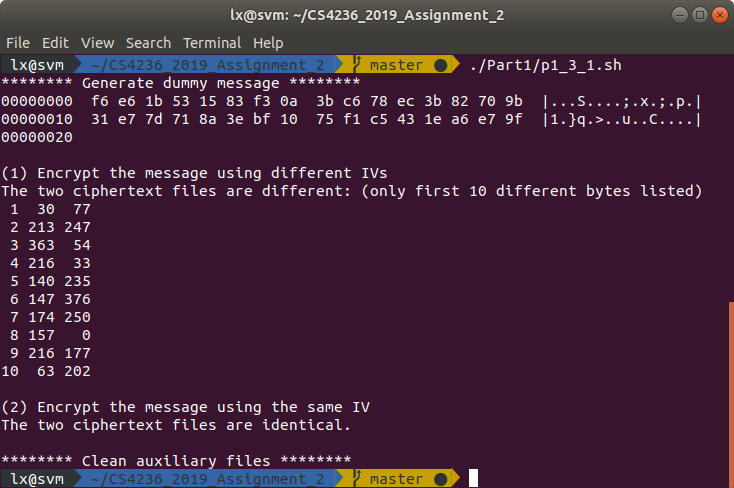
\includegraphics[width=\columnwidth]{resources/p1_3_1.png}
\caption{
    Content in file \texttt{Part1/p1\_3\_1.sh} is listed in Appendix \ref{code:1_3_1}
}
\label{fig:p1_3_1}
\end{figure}

From the outputs, it can be seen that reusing IV under the same key to encrypt the same message leads to the same ciphertext.

CPA-security requires that the encryption scheme should be probabilistic. 
A probabilistic function has to be able to get access to a randomness source.
In the encryption schemes we used, IV is the only source of randomness.
Hence if we reuse the IV, the probabilistic function falls back to a deterministic function.

Therefore, in order to keep the encryption scheme produces different ciphertext for the same plaintext, IV can never be reused.

\subsubsection{}
Yes, he/she can decrypt other messages that are not longer than the known message. Screenshot of the commands and outputs is as Fig.\ref{fig:p1_3_2}.

\begin{figure}[t!]
\centering
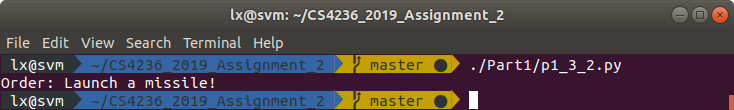
\includegraphics[width=\columnwidth]{resources/p1_3_2.png}
\caption{
    Content in file \texttt{Part1/p1\_3\_2.sh} is listed in Appendix \ref{code:1_3_2}
}
\label{fig:p1_3_2}
\end{figure}

If we use CFB mode (Fig.\ref{fig:CFB_encryption}) instead of OFB mode, we can only get the first block of a new message.

\begin{figure}[ht]
\centering
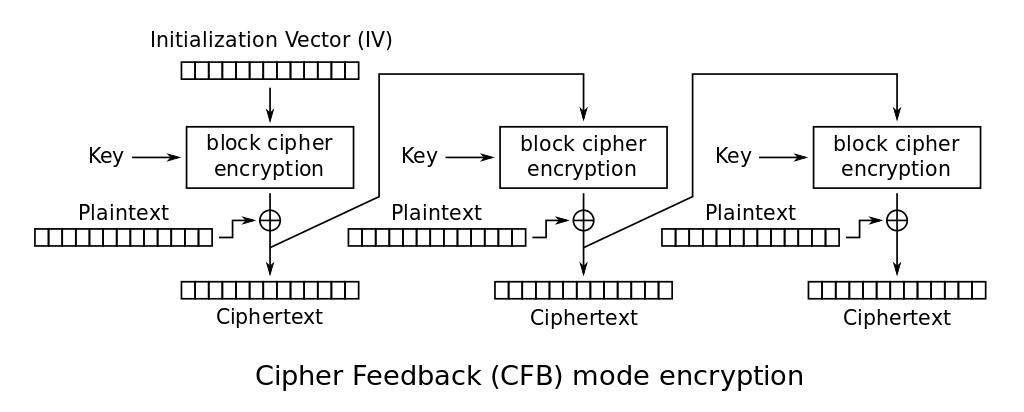
\includegraphics[width=\columnwidth]{resources/CFB_encryption.png}
\caption{
    Cipher Feedback (CFB) mode encryption \protect\footnotemark
}
\label{fig:CFB_encryption}
\end{figure}

\footnotetext{The picture comes from \texttt{https://bit.ly/1CoRiM0}}

With CFB mode, we can decrypt any message no longer than the known message because CFB generates a completely the same random stream with the same IV and xor the random stream with plaintext.

While in OFB mode, the random stream is generated not only from the IV, but also influenced by the previous block of message. Hence although the IV and the key are the same, it can generate different random stream from different messages.

But we can still get the first block of message because $m_0 \oplus c_0$ always equals to $F_k(IV)$. This is sufficient to win the CPA game.

\subsubsection{}

Screenshot of the commands and outputs is as Fig.\ref{fig:p1_3_3}.

Since the message is shorter than a block, we only consider the message and ciphertext with only one block.
In CBC mode (Fig.\ref{fig:CBC_encryption}), the first block of ciphertext 
$$c := F_k(IV \oplus m)$$
Thus knowing IV, we can keep the ciphertext identical by holding $IV \oplus m$ a constant.

\begin{figure}[t!]
\centering
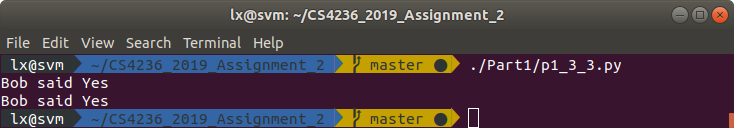
\includegraphics[width=\columnwidth]{resources/p1_3_3.png}
\caption{
    Content in file \texttt{Part1/p1\_3\_3.sh} is listed in Appendix \ref{code:1_3_3}
}
\label{fig:p1_3_3}
\end{figure}

\begin{figure}[ht]
\centering
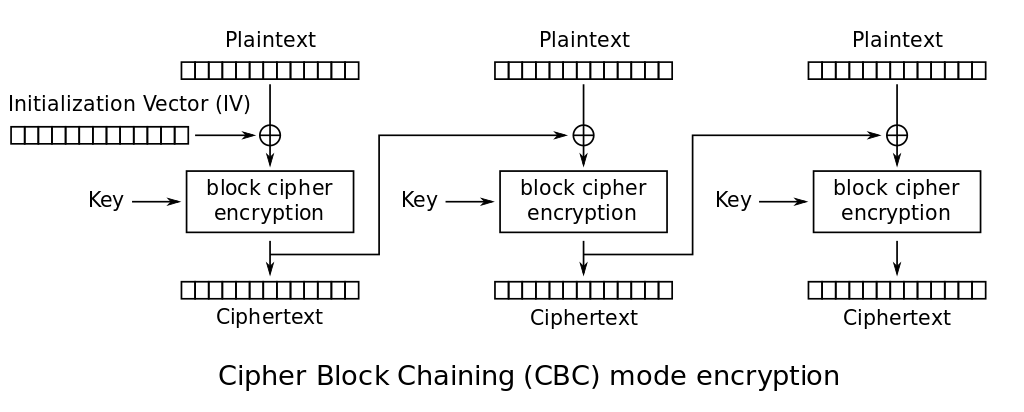
\includegraphics[width=\columnwidth]{resources/CBC_encryption.png}
\caption{
    Cipher Block Chaining (CBC) mode encryption \protect\footnotemark
}
\label{fig:CBC_encryption}
\end{figure}

\footnotetext{The picture comes from \texttt{https://bit.ly/1CoRiM0}}

To solve this problem, we can keep $IV_1 \oplus m = IV_2 \oplus m'$, where $m$ is \texttt{Yes} or \texttt{No}, $IV_1$ and $IV_2$ are known value. Thus
$$ m' = m \oplus IV_1 \oplus IV_2 $$
can be easily constructed. Then we ask Bob to encrypt the $m'$ and check if the response $C$ equals to the ciphertext $C_1$ we already known. If $C = C_1$, $m$ is exactly the message Bob sent just now.
